\documentclass[a4paper,11pt]{article}
\pagenumbering{arabic}
\usepackage{../environment}

\begin{document}

\begin{center}
    \huge{Solutions to Sheet 3}
\end{center}

\exercise{1}
\begin{enumerate}
    \item Show that $\cO_K^\times = \{x \in \cO_K \mid \Norm_{K/\Q} = \pm 1\}$.
    \item Suppose that $K = \Q(\sqrt m)$ for some negative squarefree integer
        $m$. Determine $\cO_K^\times$. 
\end{enumerate}

\textbf{Solution.}
\begin{enumerate}[wide, labelindent=0pt]
    \item We know from the lecture that for any $x \in \cO_K$, the norm
        $\Norm_{K/\Q}(x)$ lies in $\Z$. It is easy to check (for example by 
        defining the norm via the determinant) that the norm induces a
        homomorphism of groups $\Norm_{K/\Q}: \cO_K^\times \to \Z^\times$.
        This shows that units have norm $\pm 1$. 

        For the reverse inclusion, there are at least three solutions. 
        One could argue that for $x \in \cO_K$ with norm $\pm 1$, $\mu_x: \cO_K
        \to \cO_K$ (given by $\mu_x(a) = ax$) has determinant $\pm 1$, hence is
        invertible as a $\Z$-module homomorphism. Now the inverse comes from
        $x^{-1} \in K$, which now has to lie in $\cO_K$ (after some
        argumentation). Alternatively one can use the fact that $$\NormKQ(x) =
        \prod_\sigma \sigma(x) = x \prod_{\sigma \neq \sigma_0} \sigma(x) = \pm
        1,$$ where $\sigma$ runs over all inclusions of $K$ into its algebraic
        closure. 

        The coolest solution (of the ones I know and in my naive opinion) uses the fact that
        $\NormKQ(x)$ is the $0$-th coefficient of the minimal polynomial of
        $x$. The minimal polynomial yields an equation
        \begin{equation*}
            x^d + a_{d-1}x^{d-1} + \dots + a_1 x + a_0 = x^d + a_{d-1}x^{d-1} + \dots + a_1 x \pm 1 = 0,
        \end{equation*}
        and we find
        \begin{equation*}
            x\underbrace{(x^{d-1} + a_{d-1}x^{d-2} + \dots + a_2 x + a_1)}_{= \mp x^{-1} \in \cO_K} = \mp 1.
        \end{equation*}
    \item 
        Note that $K/\Q$ is always an imaginary extension, so there is an
        embedding $K \inj \C$ (well-defined up to complex conjugation) and
        the unique non-trivial element $\sigma \in \Gal(K/\Q)$ is given by
        complex conjugation. Moreover, the norm is simply given by the square
        of the complex absolute value.

        In what follows, we'll always consider $K$ a subfield of $\C$. By part 1, we know
        that all units have absolute value $1$, hence they lie on the unit circle. 
        Furthermore, we also know that any $x \in \cO_K$ has 
        $\Tr_{K/\Q}(x) = 2 \Re x \in \Z$. These conditions are quite restrictive!
        \begin{figure}[H]
        \centering
        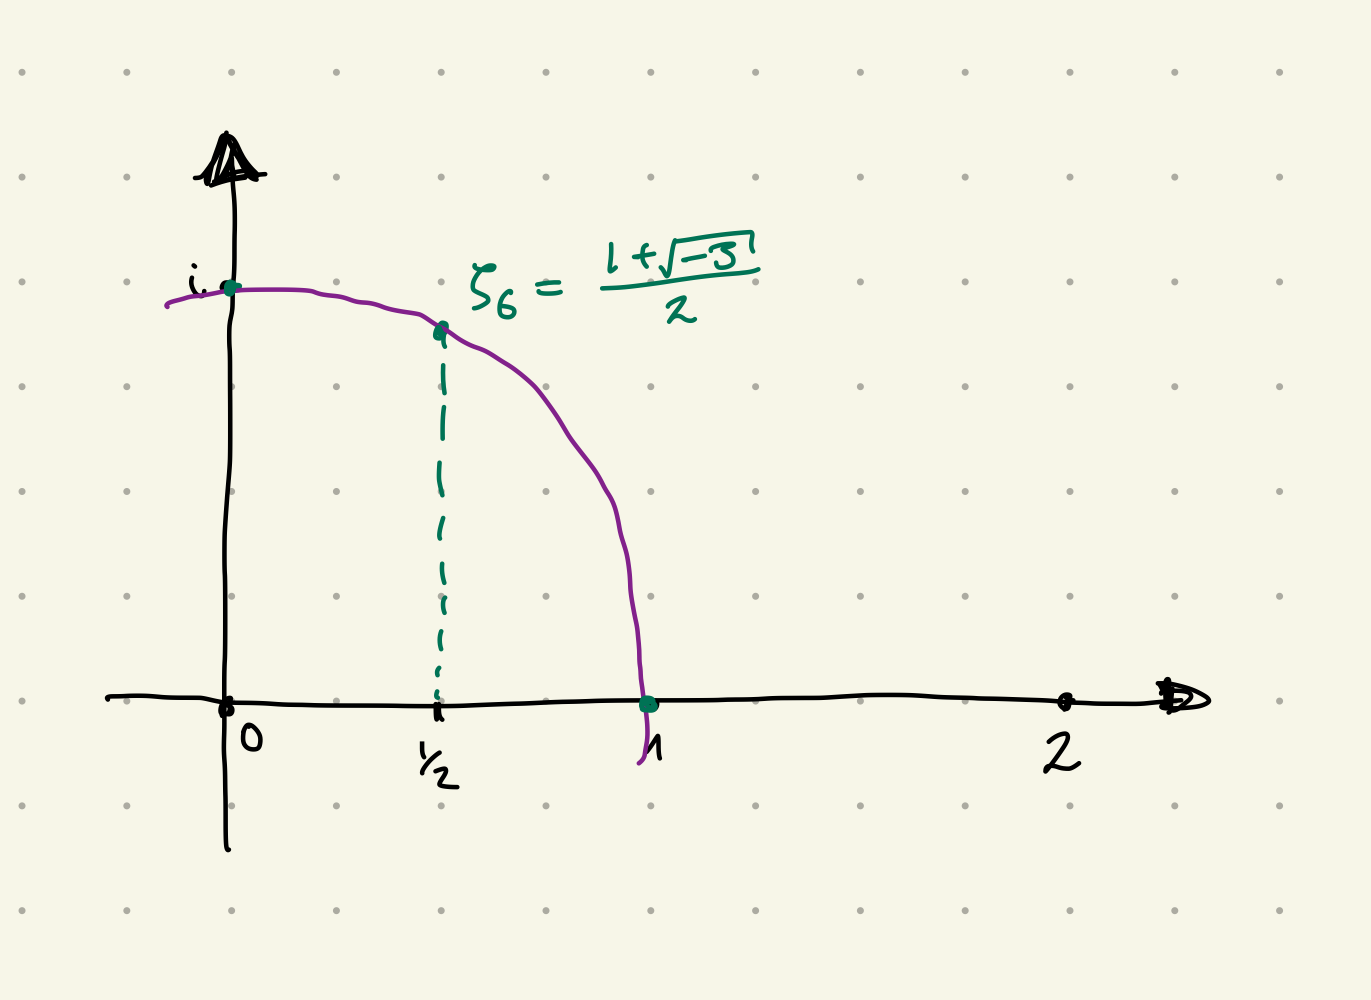
\includegraphics[width = 7cm]{ROU.jpg}
        \caption{The only points that have a chance of lying in $\cO_K^\times$ are 
        $\{\pm 1, \pm \ic, \pm \zeta_6, \pm \zeta_3\}$.}
        \end{figure}
        In fact one quickly verifies that the points $\{\pm 1, \pm \ic, \pm
        \zeta_6, \pm \zeta_3\}$ are the only points on the unit circle with 
        real value $\in \frac 12 \Z$. 
        We have seen before that $\ic \in \cO_K$ if $m = -1$ and 
        $\zeta_6^\Z \subset \cO_K$ if $m = -3$.  
        
        Finally, it is not hard to see that two non-isomorphic quadratic number
        fields have trivial intersection after choosing embeddings into $\C$. This follows
        from the fact that degree-2 extensions don't have intermediate extensions, and
        that $\Q(\sqrt m)$ and $\Q(\sqrt {m'})$ are non-isomorphic if $m \neq m'$ 
        (they have different discriminant).
        This finishes the characterization of the units
        the ring of integers of $\Q(\sqrt m)$ for negative square-free integers $m$. 
        It is given by the following subgroup of the multiplicative group of
        complex numbers:
        \begin{equation*}
            \cO_{\Q(\sqrt m)}^\times = \begin{cases}
                \ic^\Z \cong \Z/4\Z, &\text{ if }m = -1\\
                \zeta_6^\Z \cong \Z/6\Z, &\text{ if }m = -3\\
                (-1)^\Z \cong \Z/2\Z, &\text{ otherwise. }
            \end{cases}
        \end{equation*}
\end{enumerate}

\exercise{2}
Let $K$ and $L$ be number fields and let $\phi: K \to L$ be a ring homomorphism.
Show that $\phi(\cO_K) \subset \cO_L$.

\textbf{Solution.} We know that $\cO_L$ is the integral closure of $\Z$ in $L$. This
means $\cO_L$ is the subring of elements in $L$ that arise as roots of polynomials
in $\Z$. The same is true for $\cO_K$ in $K$. If any $x \in \cO_K$ is a root of a
monic polynomial $f_x(T) \in \Z[T]$. Then $\phi(x) \in L$ is a root of $f$ as well,
as $f(\phi(x)) = \phi(f(x)) = 0$ (remember that any ring morphism is a
homomorphism of abelian groups. In particular, $\phi$ is the identity
on $\Z$ and thereby does not change the coefficients of $f$).

\exercise{3}
Let $m \in \Z \setminus \{0, \pm 1\}$ be a squarefree integer. Using Eisenstein's
criterion, one shows that $X^3 -m \in \Q[X]$ is irreducible (you do not need to check
this). Set $K = \Q[X]/(X^3-m \Q[X])$, we write $x$ for the image of $X$ in $K$
so that $x^3 = m$. 
\begin{enumerate}
    \item Show that $\Delta_{K/\Q}(1,x,x^2) = -3^3 m^2$.
    \item Let $a,b,c \in \Q$. Compute $\Norm_{K/\Q}(a + bx + cx^2)$.
\end{enumerate}

\textbf{Solution.} 
\begin{enumerate}[wide, labelindent=0pt]
    \item Fix a inclusion $K \inj \overline \Q$ of $K$ in the algebraic closure of $\Q$.
        There are two other inclusions of $K$ into $\overline \Q$, namely those given by
        morphism sending $x$ (a primitive element of $K$) to $\zeta_3 x$ and
        $\zeta_3^2 x$ (here we also fixed $\zeta_3 \in \overline \Q$. By Lemma
        1.32 in the script we obtain
        \begin{equation*}
            \Delta_{K/\Q}(1,x,x^2) = \det \begin{pmatrix}
                                            1 & x & x^2 \\
                                            1 & \zeta_3 x & \zeta_3^2 x \\
                                            1 & \zeta_3^2 x & \zeta_3 x^2
                                          \end{pmatrix}^2.
        \end{equation*}
        The determinant of the matrix is readily computed to $3x^3(\zeta_3^2 - 
        \zeta_3)$, which has square $9x^6(-3) = -3^3m^2$, as desired.

    \item Let $\alpha = a + bx + cx^2$. Let $B$ be the basis $(1,x,x^2)$ of $K$
        as a $\Q$ vector space. Then $\alpha$ sends $1$ to the vectors
        $(a,b,c)$, $x$ to the vector $(mc, a, b)$ and $x^2$ to the vector
        $(mb, mc, a)$. We find that as a matrix with respect to $B$, 
        multiplication by $\alpha$ is given by
        \begin{equation*}
            \begin{pmatrix} 
                a  & mc & mb \\
                b  & a  & mc  \\
                c  & b  & a
            \end{pmatrix},
        \end{equation*}
        and the determinant of this matrix is (hopefully)
        \begin{equation*}
            a^3 + mb^3 + m^2 c^3 - 3mabc.
        \end{equation*}
        This is $\NormKQ(\alpha)$.
\end{enumerate}

\exercise{4}
To the right, you do not see the flag of Nepal. The ration of its height to its 
width is equal to a number $\alpha \in \R$ such that $K \coloneqq \Q(\alpha)
= \Q(\sqrt{59-24\sqrt 2})$.
\begin{enumerate}
    \item Show that $[K:\Q]=4$ and that 
        \begin{equation*}
            \left(1, \sqrt{59 - 24\sqrt 2}, \sqrt 2, \sqrt2 \sqrt{59- 24\sqrt 2}
                \right)
        \end{equation*}
        is a $\Q$-basis of $K$.
    \item Show that $\beta \coloneqq (-1 + \sqrt{59 - 24\sqrt 2}/\sqrt 2 \in \cO_K$. 
    \item Set $F = \Q(\sqrt 2)$. Show that $2(59- 24\sqrt 2) \cO_K \subset
        \cO_F[\beta]$. 
\end{enumerate}

\textbf{Solution.}
\begin{enumerate}[wide, labelindent=0pt]
    \item First, after squaring twice we find that $\alpha$ is a root of the
        polynomial
        \begin{equation*}
            f(X) = X^4 - 118X^2 + 2329.
        \end{equation*}
        We find that $f$ is irreducibe by seeing that there are no rational roots to $f$
        (we only have to check divisors of $2329$), and the approach
        \begin{equation*}
            f(X) = (aX^2 + bX + c)(dX^2 + eX + f)
        \end{equation*}
        reveals that there is no factorization.\footnote{Alternatively, ask Wolframalpha
        or smth idk.} This shows that 
        $(1, \alpha, \alpha^2, \alpha^3)$ is a basis for $L/\Q$. Note that
        $\Q(\alpha^2) = \Q(\sqrt 2)$. This shows that $(1, \alpha, \sqrt 2, \sqrt 2 \alpha)$
        is a basis too.
    \item Note that $\beta^2 = 30 - 12\sqrt 2 \in \cO_K$ and that $\beta = \sqrt 2^{-1}
        (-1 + \alpha) \in K$. As $\cO_K$ in integrally closed in $K$, this implies that 
        $\beta \in \cO_K$. Indeed, $\beta \in K = \Frac (\cO_K)$ is a root of the monic
        polynomial $T^2 - \beta^2 \in \cO_K[T]$.
    \item As $(1, \beta)$ is an $F$-basis for $K$, the lecture notes reveal the
        fact that $$\Delta_{K/F}(1, \beta) \cO_K \subseteq \cO_F + \beta \cO_F
        \subseteq \cO_F[\beta].$$ So perhaps calculating
        the discriminant solves the exercise in an instant. 
        The minimal polynomial of $\alpha$ over $F$ is given by $T^2 - (59 -
        24\sqrt 2) = 0$, which shows that $\Gal(K/F)$ is the group of order $2$
        generated by the $F$-linear $K$-automorphism $\sigma$ that sends $\alpha$ to 
        $-\alpha$ (i.e., $\sigma(x + \alpha y) = x - \alpha y$). Writing $\beta = \frac {1 - \alpha}{\sqrt 2}$, we find that 
        \begin{equation*}
            \Delta_{K/F}(1, \beta) = \det \mat 1 \beta 1 {\sigma(\beta)}^2
            = (\sigma(\beta) - \beta)^2 = 2 \alpha^2.
        \end{equation*}
        This is exactly what we needed. The result from the lecture now implies
        \begin{equation*}
            \cO_F[\beta] \supseteq \Delta_{K/F}(1, \beta) \cO_K
            = 2 \alpha^2 \cO_K = 2(59 - 24\sqrt 2) \cO_K.
        \end{equation*}

        
\end{enumerate}


\contactend

\end{document}
%This can also be written as $g(X^2)$. We quickly find four real roots of $f$.
%        Obviously $f(-\alpha) = 0$. But also, as $\alpha^2 = 59 - 24 \sqrt2 \in \Q(\sqrt 2)$
%        satisfies $g(\alpha^2) = 0$, we find that $0 = g(\sigma(\alpha^2)) =
%        f(\sigma(\alpha))$, where $\sigma: \Q(\sqrt 2) \to \Q(\sqrt 2)$ is the
%        nontrivial element sending $\sqrt 2$ to $-\sqrt 2$. Hence $f$ has four
%        real roots
%        \begin{equation*}
%            \alpha_1 = \sqrt{59- 24\sqrt 2}, \quad 
%            \alpha_2 = -\sqrt{59- 24\sqrt 2}, \quad 
%            \alpha_3 = \sqrt{59 + 24\sqrt 2}, \quad 
%            \alpha_4 = -\sqrt{59 + 24\sqrt 2}. 
%        \end{equation*}
%        These are all quickly verified to be irrational.
%        
%
